\documentclass[twocolumn]{IEEEtran}
\usepackage{graphicx}
\usepackage[utf8x]{inputenc}
\usepackage{times}
\usepackage{amssymb,amsfonts}
\usepackage{pict2e}
\usepackage{float}
\usepackage[all]{xy}
\usepackage{graphics,graphicx,color,colortbl}
\usepackage{subfigure}
\usepackage{wrapfig}
\usepackage{multicol}
\usepackage{cite}
\usepackage{url}
\usepackage[tbtags]{amsmath}
\usepackage{amsmath,amssymb,amsfonts,amsbsy}
\usepackage{bm}
\usepackage{listings}
\usepackage{algorithm}
\usepackage{algorithmic}
\usepackage[centerlast, small]{caption}
\usepackage[colorlinks=true, citecolor=blue, linkcolor=blue, urlcolor=blue, breaklinks=true]{hyperref}
\hyphenation{ele-men-tos}

\begin{document}
\title{Introducción a la Plataforma LEGO Mindstorms}
\author{Israel Ricardo Bernal Sanchez Código: $261613$\\
	Felipe Castañeda Prieto Código $285728$\\
	David Ricardo Martínez Hernández Código: $261931$\\
	Oscar Andrés Urbano Vallejo Código: $261683$}
\maketitle
\markboth{Universidad Nacional de Colombia}{}
\floatname{algorithm}{Algoritmo}
\begin{abstract}
 Se diseñaron $2$ diferentes algoritmos para que el motor se comportara como una señal diente de sierra, el primer controlaba un motor de acuerdo al numero de pulsaciones al momento de girar, el segundo lo hacia por medio de velocidad, finalmente se diseño un algoritmo que utilizara un sensor, para este caso fue el sensor de luz, que media la intensidad de luz y el motor giraba en ausencia de luz.
\end{abstract}

\begin{keywords}
 Algoritmo, Brick, LEGO, Lenguaje, NXC, Servomotor.
\end{keywords}

\section{Introducción}
\noindent
A lo largo del curso de control se va hacer uso de unas herramientas de programación e implementación, estas son la plataforma de programación conocida como: \textbf{\textit{``Bricx Command Center''}} y  la herramienta de implementación \textbf{\textit{``Lego Midstorms NXT''}}. En esta práctica se introducen los conceptos básicos de dichas herramientas y se describen algunos de sus componentes principales. 

\section{Procedimiento}
\subsection{Introducción al Hardware}
\begin{enumerate}
 \item Investigar sobre las características técnicas de los elementos internos que componen la unidad básica de procesamiento (Brick) como la capacidad en memoria Flash y Ram, velocidad de procesamiento y protocolo de comunicación del procesador y coprocesador.\\\\
La unidad básica de procesamiento se compone de dos procesadores:
El \textbf{procesador principal}: Encargado del manejo de la alimentación, de la creación de señales, de la  conversión Análoga/Digital, además de la comunicación con el display, el sonido y el dispositivo Bluetooth.\\
Procesador ATMEL ARM7 de $32$ bits ($AT91SAM7S256$). Cuenta con $256$ Kbytes de memoria Flash y $64$ Kbytes de memoria RAM velocidad de procesamiento de $48$ MHz.\\
El \textbf{Co-Procesador}: Que se comunica con el procesador principal  por medio del protocolo $I2C$ (\textit{Inter Integrated Circuit}) a una velocidad de $380$  kbytes/s.  La comunicación es realizada mediante la actualización de $2$ registros de memoria cada $2$ ms.\\
Procesador \textbf{ATMEL AVR} de $8$ bits ($ATmega48$). Cuenta con $4$ Kbytes de memoria Flash y $512$ bytes de memoria RAM, velocidad de procesamiento de $8$ MHz.\\
\item Identificar las limitaciones en alimentación y velocidad de comunicación de los puertos de entrada y salida del Brick.\\\\
Los puertos de entrada y salida del Brick pueden ser alimentados con una corriente máxima de $700$ mA y de $1$ A pico, el voltaje no supera los $9$ V esto en vista de que el brick utiliza $6$ pilas de $1.5$ V de alimentación.\\
La comunicación con los puertos de entrada se hace con una frecuencia máxima de muestreo de las señales de $333$ Hz.\\
\item  Investigar sobre las características técnicas de los siguientes sensores: ultrasonido, EOPD, color, giroscopio, acelerómetro, sensor de contacto (Touch), brújula magnética (Compas).\\\\
\textbf{Sensor de Ultrasonido:} Este sensor se comunica con el Brick mediante el Protocola $I2C$, funciona enviando señales sónicas y analizando su eco, para determinar la distancia a la que se encuentra un objeto (obstáculo o pared), es capaz de detectar objetos que se encuentren desde $0$ a $255$ cm de distancia, con una precisión de $\pm 3$ cm.
\begin{figure}[H]
	\centering
		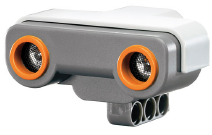
\includegraphics[scale=0.6]{sonido.png}
	\caption{Sensor de Ultrasonido (Tomado de \cite{page2}).}
	\label{fig1}
\end{figure}
\noindent
\textbf{EOPD:} Sensor Eléctrico de proximidad, por medio de una fuente de luz interna este sensor es capaz de detectar la presencia de un objeto o determinar cambios en la distancia al mismo con bastante precisión (es capaz de detectar objetos en distancias de hasta $20$ cm), esto depende de la forma del objeto y de  sus características de reflexión. Gracias  a que genera su propia fuente de luz este sensor filtra las señales de luz externas lo que garantiza su movilidad independientemente de la luminosidad de la zona.\\ 

\textbf{Sensor de color:} Este sensor distingue entre 6 diferentes colores, además es capaz de medir la intensidad de la luz  en un cuarto o bien la intensidad de esta reflejada en superficies de color, adicionalmente este sensor puede funcionar como una lámpara de color.
\begin{figure}[H]
	\centering
		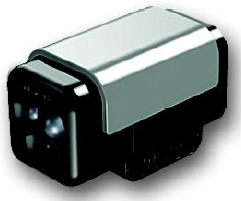
\includegraphics[scale=0.6]{color.png}
	\caption{Sensor de Color (Tomado de \cite{page2}).}
	\label{fig2}
\end{figure}
\noindent
\textbf{Giroscopio:} El sensor de giro permite medir la velocidad de rotación del robot tomando hasta $300$ muestras de dicha velocidad en un segundo, este sensor devuelve  el número de grados por segundo y la dirección de la rotación.
\begin{figure}[H]
	\centering
		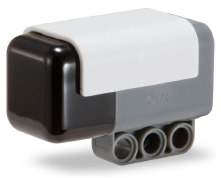
\includegraphics[scale=0.6]{rotacion.png}
	\caption{Sensor de Rotación o Giroscopio (Tomado de \cite{page2}).}
	\label{fig3}
\end{figure}

\textbf{Acelerómetro:} sensor capaz de medir aceleración en los $3$ ejes $(x, y, z)$.  La aceleración es medida en el rango de $-2g$ a $+2g$ con una resolución de aproximadamente $200$ unidades por $g$, es capaz de tomar hasta $100$ mediciones en un segundo.\\

\textbf{Sensor de Contacto:} el sensor de contacto funciona como interruptor de corriente normalmente abierto, provoca una variación de voltaje de $0$ a $5$ V cuando es activado, se activa mediante la pulsación, este puede ser utilizado como sensor de choque.
\begin{figure}[H]
	\centering
		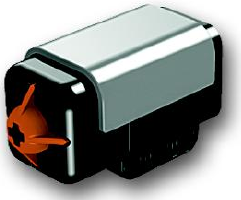
\includegraphics[scale=0.6]{tacto.png}
	\caption{Sensor de Contacto (Tomado de \cite{page2}).}
	\label{fig4}
\end{figure}
\noindent
\textbf{Brújula Magnética:} este sensor es capaz de medir el campo magnético terrestre y calcular donde está el norte magnético.  Se puede calibrar para corregir anomalías de campo magnético debidas a diferentes elementos tales como motores, baterías entre otros. La brújula magnética devuelve un valor correspondiente a la dirección actual del sensor, este valor se encuentra entre $0°$ y $359°$  y  tiene una precisión de $ \pm 1°$.  Este sensor actualiza sus medidas hasta $100$0 veces en un segundo.
\end{enumerate}

\subsection{Introducción al Software}
\begin{enumerate}
 \item  Describir la estructura básica de programación bajo lenguaje NXC en BricxCC y los diferentes tipos de variables que se pueden definir dentro de este entorno.\\\\
El programa \textbf{Bricx Comand Center} o \textbf{BricxCC} es un programa de Windows, capaz de proporcionar un ambiente integrado de desarrollo o \textbf{IDE}, para la programación de diferentes aplicaciones o dispositivos. Este  programa permite la programación de las diferentes versiones de los bloques \textbf{RCX Lego Mindstorm}, bajo diferentes tipos de lenguajes de programación como $C$, $C++$, $Pascal$, entre otros; bajo la implementación del firmware asociado al lenguaje utilizado. El bloque \textbf{NXT} es una versión mejorada de los bloques \textbf{RCX}, el cual se puede programar por medio del programa \textbf{BricxCC} usando los lenguajes \textbf{NXC (Not Exactly C)} o \textbf{Next Byte Codes (NBC)}.\\
El lenguaje de programación NXC es permite la programación del NXT, a través del compilador del lenguaje NXC que traduce el código fuente a \textbf{bytecode}, el cual recibe el bytecode interpreter que se encuentra en el NXT y es proporcionado por LEGO, para ejecutar las tareas programadas. Aunque el lenguaje NXC es bastante similar al lenguaje C, el lenguaje NXC no es un lenguaje desarrollado para propósito general, y tiene algunas restricciones y limitaciones, decido a la capacidad del bytecode interpreter.\\
La programación de NXC se realiza por medio de bloques de código y definición de variables. Los bloques de códigos pueden ser de tipo “task” o de tipo “function”, los cuales tienen sus propias características, aunque comparten estructuras comunes. \\
Los bloques \textit{``task''}  son constituidos por un nombre precedido por el identificador que constituyen el encabezado, seguido por el cuerpo del bloque en el que se ubican las declaraciones que describen la tarea a realizar. Todos los programas tienen al menos un \textit{``task''} llamado \textit{``main''}, el cual es el primero en ejecutarse cuando se corre el programa dentro del NXT.\\
El bloque \textit{``function''} es un conjunto de declaraciones que pueden ser llamadas por el código para le ejecución de tareas y obtención de un resultado, lo cual resulta bastante importante y facilita la implementación de tareas complicadas, que resultarían en código extenso. Las funciones son capaces de recibir varios argumentos, que permiten ejecutar sus funciones y retornar un valor, que está definido entre los tipos de variables que se pueden manejar.\\
NXC es un lenguaje de programación sensible al tamaño, por lo que diferencia entre mayúsculas y minúsculas para identificar los comandos. Este lenguaje muestra bastantes similaridades con la estructura de programación del lenguaje C, como permitir la realización de comentarios dentro del programa mediante el uso de ``$/**/$'' o ``$//$''.\\
Las variables que pueden ser definidas en NXC son variables \textit{bool, byte, char, int, short, long, unsigned, float, string, Structures y Arrays}. Las variables bool ocupa $8$ bits de memoria y toma los valores  de \textit{``true''} o \textit{``false''}. Los tipos de variables utilizados para almacenar números  de menor a mayor capacidad son byte ($8$-bit), short ($16$-bit), int ($32$-bit), long ($64$-bit) y float ($32$-bit), donde los float permiten el almacenamiento de números con hasta siete dígitos decimales. La palabra clave \textit{``unsigned''} modifica los tipos int, long y char, para almacenar los valores sin observar el bit de signo lo que permite un mayor almacenamiento de enteros positivos. La variable char permite guardar en 8 bits un solo carácter que toman internamente los valores $ASCII$, los tipo srting son arreglos de bytes que permiten almacenar más caracteres en una sola variables. Las constantes numéricas pueden ser escritas en decimal, o en hexadecimal mediante la anteposición de $0x$ a los dígitos.      \\
Las estructuras (Structures) se definen de manera similar a $C$ y cuentan con las características que  son representadas dentro de su construcción. NXC permite manejar arreglos de variables, precisando en su declaración el tipo de variable que se almacena y la cantidad de elementos que es capaz de almacenar.\\

 \item Diseñar e implementar dos algoritmos: uno que conduzca el movimiento en posición de un servomotor siguiendo el patrón de una señal diente de sierra; y otro que conduzca el movimiento en velocidad de un servomotor siguiendo el patrón de una señal diente de sierra.
\lstset{numbers=left, numberstyle=\tiny, stepnumber=1, numbersep=1pt}
\begin{lstlisting}[firstnumber=1, caption=Código Posición, label=code1]
  long j;
task main(){
  TextOut(0,50,"David 261931");
  TextOut(0,40,"Felipe 285728");
  TextOut(0,35,"Ricardo 261613");
  TextOut(0,25,"Oscar 261683");
repeat(4){
  for( int i=0; i<=100; i+=1){
// OnFwd: Acciona el motor del puerto de
// salida A
    OnFwd(OUT_A,10);
// Wait: Detiene la ejecucion del
// programa durante el tiempo determinado
    Wait(40);
// MotorRotationCount: Permite conocer la
// posicion angular del motor
    j=MotorRotationCount(OUT_A);
    TextOut(0,20,"Conteo: ");
// NumOut: Muesra el valor asignado en una
// posicion determinada
    NumOut(10,10,j);
    }
// OnRev: Acciona el motor en direccion
// contraria
  OnRev(OUT_A,90);
  Wait(400);
  }
// Off: Detiene el motor del puerto de
// salida A
  Off(OUT_A);
}
\end{lstlisting}

\lstset{numbers=left, numberstyle=\tiny, stepnumber=1, numbersep=1pt}
\begin{lstlisting}[firstnumber=1, caption=Código Velocidad, label=code1]
  long j;
task main(){
  TextOut(0,50,"David 261931");
  TextOut(0,40,"Felipe 285728");
  TextOut(0,35,"Ricardo 261613");
  TextOut(0,25,"Oscar 261683");
repeat(4){
//for: permite aumentar la velocidad del
// motor
  for( int i=0; i<=100; i+=1){
// OnFwd: Acciona el motor del puerto de
// salida A
    OnFwd(OUT_A,i);
// Wait: Detiene la ejecucion del 
// programa durante el tiempo determinado
    Wait(40);
// MotorRotationCount: Permite conocer la
// posicion angular del motor
    j=MotorRotationCount(OUT_A);
    TextOut(0,20,"Conteo: ");
    NumOut(10,10,j);
    }
// OnRev: Acciona el motor en direccion
// contraria
  OnRev(OUT_A,-10);
  Wait(40);
  }
// Off: Detiene el motor del puerto de
// salida A
  Off(OUT_A);
}
\end{lstlisting}

 \item  Diseñar e implementar un algoritmo que utilice otro sensor diferente a la posición angular del servomotor.
\lstset{numbers=left, numberstyle=\tiny, stepnumber=1, numbersep=1pt}
\begin{lstlisting}[firstnumber=1, caption=Código Sensor de Intensidad de Luz, label=code1]
  long j;
task main(){
  TextOut(0,50,"David 261931");
  TextOut(0,40,"Felipe 285728");
  TextOut(0,35,"Ricardo 261613");
  TextOut(0,25,"Oscar 261683");
while(true){
//SetSensorType: Indica el tipo de sensor
// usado y el puerto de entrada
SetSensorType(IN_1,SENSOR_TYPE_LIGHT_ACTIVE);
// Sensor: devuelve el valor leido por el
// sensor
  j=Sensor(IN_1);
  TextOut(0,20,"Conteo: ");
  NumOut(10,10,j);
  Wait(200);
    if(j<=200){
      OnFwd(OUT_A,100);
      }
    else{
      Off(OUT_A);
      }
    }
}
\end{lstlisting}
\end{enumerate}

\section{Conclusiones}
\begin{itemize}
 \item Una de las grandes ventajas del lenguaje de programación NXC es su gran similitud con C uno de los más conocidos lenguajes de programación, lo que facilita la implementación de algoritmos en dicho lenguaje.
 \item NXC además de contar con los comandos utilizados en C agrega unos cuantos comandos nuevos que facilitan diferentes tareas de programación orientadas al control, un claro ejemplo de esto es el comando repeat (Numero) utilizado para repetir una instrucción un determinado número de veces.
 \item El kit de robótica Lego Mindstorms NXT  es de gran utilidad a la hora de implementar tareas de control gracias a su gran número de componentes como sensores, actuadores etc, además de esto permite fundar solidas bases de programación y control de procesos  en quienes los utilizan.
 \item La experiencia obtenida en este laboratorio con la señal de posición en forma de Diente de Sierra muestra la importancia de realizar una correcta calibración de los sensores y actuadores con los que se va a trabajar, esto en pro de conseguir los mejores resultados a la hora de la implementación de los futuros algoritmos de control.
\end{itemize}

\bibliographystyle{ieeetran}
\begin{thebibliography}{99}

\bibitem{chen} Chen, Chi-Tsong.
{\em "`Analog and Digital Control System Desing: Transfer-Function, State, Space and Algebraic Methods"'}.
Saunders College Publishing, 1993.

\bibitem{kuo} Kuo, C. Benjamin.
{\em "`Sistemas Automáticos de Control"'}.
Pentice Hall Hispanoamerica, Séptima Edición, 1996.

\bibitem{ogata} Ogata, Katsuhiko.
{\em "`Ingeniería De Control Moderna"'}.
Pearson Educación, Tercera Edición, 1998.

\bibitem{page1} Sitio Web: \url{http://us.mindstorms.lego.com/en-us/support/buildinginstructions/8547/8547%20User%20Guide%20English.aspx}, visitado el domingo 11 de Agosto

\bibitem{page2} Sitio Web: \url{http://cache.lego.com/Media/Download/Mindstorms2BuildingInstructions/otherfiles/downloadA0B7A698E231D3E619C43ECCFFE2F27F/8547UserGuideEnglish_PDF.pdf}, Manual de usuario de LEGO Mindstorms.

\bibitem{page3} Sitio Web: \url{http://bricxcc.sourceforge.net/nbc/nxcdoc/NXC_Guide.pdf
http://bricxcc.sourceforge.net/nbc/nxcdoc/NXC_Guide.pdf}, visitado el viernes 18 de Agosto.
\end{thebibliography}
\end{document}